\section{Methodik}
\label{Methodik}
Die Lösung der Problemstellung wird anhand einer exemplarischen Implementierung eines drahtlosen Fußschalters durchgeführt. Dieser soll als Produkt in das Sortiment der Hoffmann Group eingeführt werden, weswegen die Implementierungen, die für diese Arbeit durchgeführt wird, über eine prototypische Implementierung hinausgehen. Dies zeigt sich insbesonderes in der ausgiebigen Analyse der Probleme, die während der Umsetzung aufgetreten sind. 

\subsection{Evaluierung der Dongle-App}
Der Prototyp der Dongle-App zeigt, dass die Umsetzung der funktionalen Anforderungen technisch möglich sind. Für den Fußschalter sollen sie evaluiert und wenn nötig verbessert werden.\\
Durch die Entwicklung des Fußschalter entstehen drei verschiedene Projekte, deren Code sich jeweils stark überschneidet, jedoch getrennt werden müssen. Dabei müssen Updates und Änderungen für eines der Projekte mit einem möglichst geringen Aufwand auch in die anderen übernommen werden, während die in den unterschiedlichen Projekte benötigte Peripherie nur in diesen initialisiert werden soll. Daher muss evaluiert werden, welche Möglichkeiten zur Verfügung stehen die einzelnen Projekte voneinander zu trennen und die Entscheidung getroffen werden welche umgesetzt werden soll.\\
Der Verbindungsaufbau mit einem auf \ac{BLE} und \ac{GATT} beruhenden Gerät wird normalweise in mehreren Schritten durchgeführt. Der erste Schritt ist das Erkennen des advertisenden Gerätes. Danach wird die Verbindung geschlossen. Nach dem Schließen der Verbindung wird die Service-Discovery durchgeführt. Dabei muss der \ac{HCT}-Service mit den beiden Characteristiken RX und TX gefunden werden und sich für die RX-Characteristik subscribed werden, erst nach der erfolgreichen Subsription kann mit dem Geräte das \ac{HCT}-Protokoll gesprochen werden. Diese Schritte werden bisher nicht vollständig in der Dongle-App abgebildet werden. Für den Fußschalter muss untersucht werden, ob die bestehende Abbildung der Verbindungschritte verbessert werden kann.\\
Jede Nachricht die über \ac{BLE} gesendet wird braucht Rechenleistung und Energie und steigt mit der Anzahl der verbundenen Geräte linear an. Auch bier besteht Verbesserungspotenzial in der Dongle-App, da die Implementierung der Messergebisabfrage mit Schwierigkeiten verbunden war und die Lösung dieser Probleme vorallem in Hinsicht auf eine schnelle Fertigstellung des Proof-of-concept Prototyps entwicklet wurde. Für den Fußschalter soll einen effizientere Lösung entwickelt werden. In Kapitel \ref{ÜberarbeitungDongleApp} werden diese Optimierungen für die Dongle-App durchgeführt.

\subsection{Konfiguration des Fußschalters}
Die durch den Fußschalter gesammelten Daten sollen in einem möglichst breiten Spektrum zur Weiterverarbeitung bereitgestellt werden. Auch durch den Fußtaster gegebene Funktionalitäten, wie z.B. das Ausgeben eines spezifischen und konfigurierbaren Zeichens bei Betätigung, sollen abgedeckt werden. Der Anwender muss die Art wie der Fußschalter eingesetzt wird, spezifizieren können und die Datenverarbeitung innerhalb der Anwendung des Fußschalters muss dementsprechend flexibel und anpassbar gestaltet werden. Eine weitere Herausforderung dabei ist, dass dem Anwender nur äußerst begrenzte Interaktionsmöglichkeiten mit dem Fußschalter zu Verfügung stehen.\\
Um diesen Anforderungen gerecht zu werden, wurde die Entscheidung getroffen Messmodi einzuführen. Der Messmodus, in dem der Fußschalter arbeiten soll, kann in einer zusätzlichen globalen Konfigurationsdatei angegeben werden und legt fest welche Funktionalität bereitgestellt wird. Dadurch wird dem bereits bei der Konfiguration der zu verbindenden Geräte verwendeten Schema gefolgt, dass der Fußschalter durch die Dateien, die im Massenspeichermedium liegen, konfiguriert wird und liefert dem Anwender visuelles Feedback über die derzeitigen Einstellungen. Durch Kommentare in der Konfigurationsdatei können zudem die möglichen Einstellungsoptionen dem Anwender leicht zugänglich gemacht werden.\\
Eine grundlegend andere Möglichkeit verschiedenste Einstellungen durchzuführen, ist durch Kombinationen aus langen und kurzen Betätigungen des Fußtasters nicht sichtbare Menüs aufzurufen und mit Hilfe einer Bedienungsanleitung die gewünschten Optionen auszuwählen. Auch wenn diese Möglichkeit in Produkten wie Kaffeemaschinen oder digitalen Weckern eine weite Verbreitung findet, hat sie den entscheidenden Nachteil, dass der Anwender keinerlei grafisches Feedback bekommt. Auch ist für eine solche Implementierung von Vorteil, wenn das Gerät mehrere Tasten besitzt, um die Wahrscheinlichkeit des versehentlichen Ansteuern von Menüs und Umkonfiguration des Fußschalters zu minimieren. Aufgrund des grafischen Feedbacks und der Konsistenz mit der Konfiguration der zu verbindenden Geräte wird die erste Möglichkeit dazu umgesetzt. In Kapitel \ref{Messmodi} wird die Umsetzung der Messmodi beschrieben.\\
Aus der Konfiguration des Messmodus über eine Konfigurationsdatei entsteht die Problemstellung, dass festgestellt werden muss, dass eine Umkonfiguration durchgeführt wurde. Zum Beginn dieser Arbeit muss der Dongle jedes Mal, wenn die Konfigurationsfiles geändert wurden, aus- und wieder eingesteckt werden, damit die Anwendung neugestartet wird und die Dateien erneut eingelesen werden. Der Fußschalter bekommt jedoch bei Verlust der \ac{USB}-Verbindung automatisch den benötigten Strom von seiner eingebauten Batterie, weswegen ein harter Reset durch den Anwender nicht ohne weiteres möglich ist. In Kapitel \ref{UberarbeitungMSC} werden daher Möglichkeiten evaluiert, wie die Anwendung des Fußschalters Änderungen an den Konfigurationsdateien detektieren kann, damit anschließend automatisch ein Neustart des Geräts durchgeführt wird.

\subsection{Einbindung der Werkzeuge}
Mit dem Fußschalter soll ein Gerät geschaffen werden, dass die Messdaten von einem möglichst breiten Spektrum an Werkzeug sammeln kann. Dabei bestehen grundlegende Abhängigkeiten zum Medium der Verbindung (\ac{BLE}) und zum Protokoll (\ac{HCT}), das über diese Verbindung gesprochen wird. Diese werden aufgrund der Spezifikation des Fußschalters, Messgeräte über das \ac{HCT}-Protokoll anzubinden, nicht aufgelöst. Jedoch sollen für diese Geräte Mechanismen geschaffen werden, um sie möglichst vollständig einzubinden und für in Zukunft entwickelte Geräte erweiterbar zu bleiben. Dabei müssen außerdem die oft sehr unterschiedlichen Funktionen der Geräte im Fußschalter zu vereinen.\\
Bei der Einbindung von neuen Geräten in die Anwendung des Fußschalters zeigt sich schnell ein grundlegendes Problem. Während das \ac{HCT}-Protokoll den Verbindungsaufbau vollständig abstrahiert und damit alle \ac{HCT}-fähigen Geräte verbunden werden können, bestehen in den Messdaten messgerätspezifische Unterschiede. So besitzt das \ac{HCT}-Protokoll generischen Datenblöcke, die für alle Geräte gleich sind, jedoch befindet sich das eigentliche Messergebnis, also die spezifischen Daten, oft an einer unterschiedlichen Stelle innerhalb dieses Blocks. Daher müssen für die Einbindung eines neuen Werkzeugs, Mechanismen geschaffen werden, die eine flexible Verarbeitung der Messdaten erlauben.\\
Des Weiteren besteht zwischen Messuhren und Drehmomentschlüssel ein grundlegender funktioneller Unterschied. Zwar messen beide Geräte kontinuierlich einen Wert, jedoch ist das eigentliche Messergebnis, das ausgegeben und gespeichert wird, ein jeweils anderes. Eine Messuhr oder Messschieber zeigt ausschließlich den derzeitigen Messwert an, während der in einer bestimmten Zeit maximal erreichte Messwert von keinem Interesse ist. Das ist bei einem Drehmomentschlüssel genau andersherum, da er nachdem eine Schraube angezogen wurde, die maximal erreichte Kraft, die während der Verschraubung erreicht wurde, als Messergebnis anzeigen soll und es auch solange anzeigt, bis erneut eine Kraft am Drehmomentschlüssel anliegt. Dieses Verhalten kann in Abbildung \ref{fig:Messmittel} gesehen werden. Mit dem Drehmomentschlüssel der Marke Garant wurde eine Verschraubung durchgeführt und der Anwender muss die Senden Taste drücken um einerseits im Arbeitablauf fortzufahren und andererseits die Messung über \ac{BLE} zu senden. Der Messschieber und die Messuhr hingegen zeigen den derzeitigen Messwert an.
\begin{figure}[H] 
	\centering
	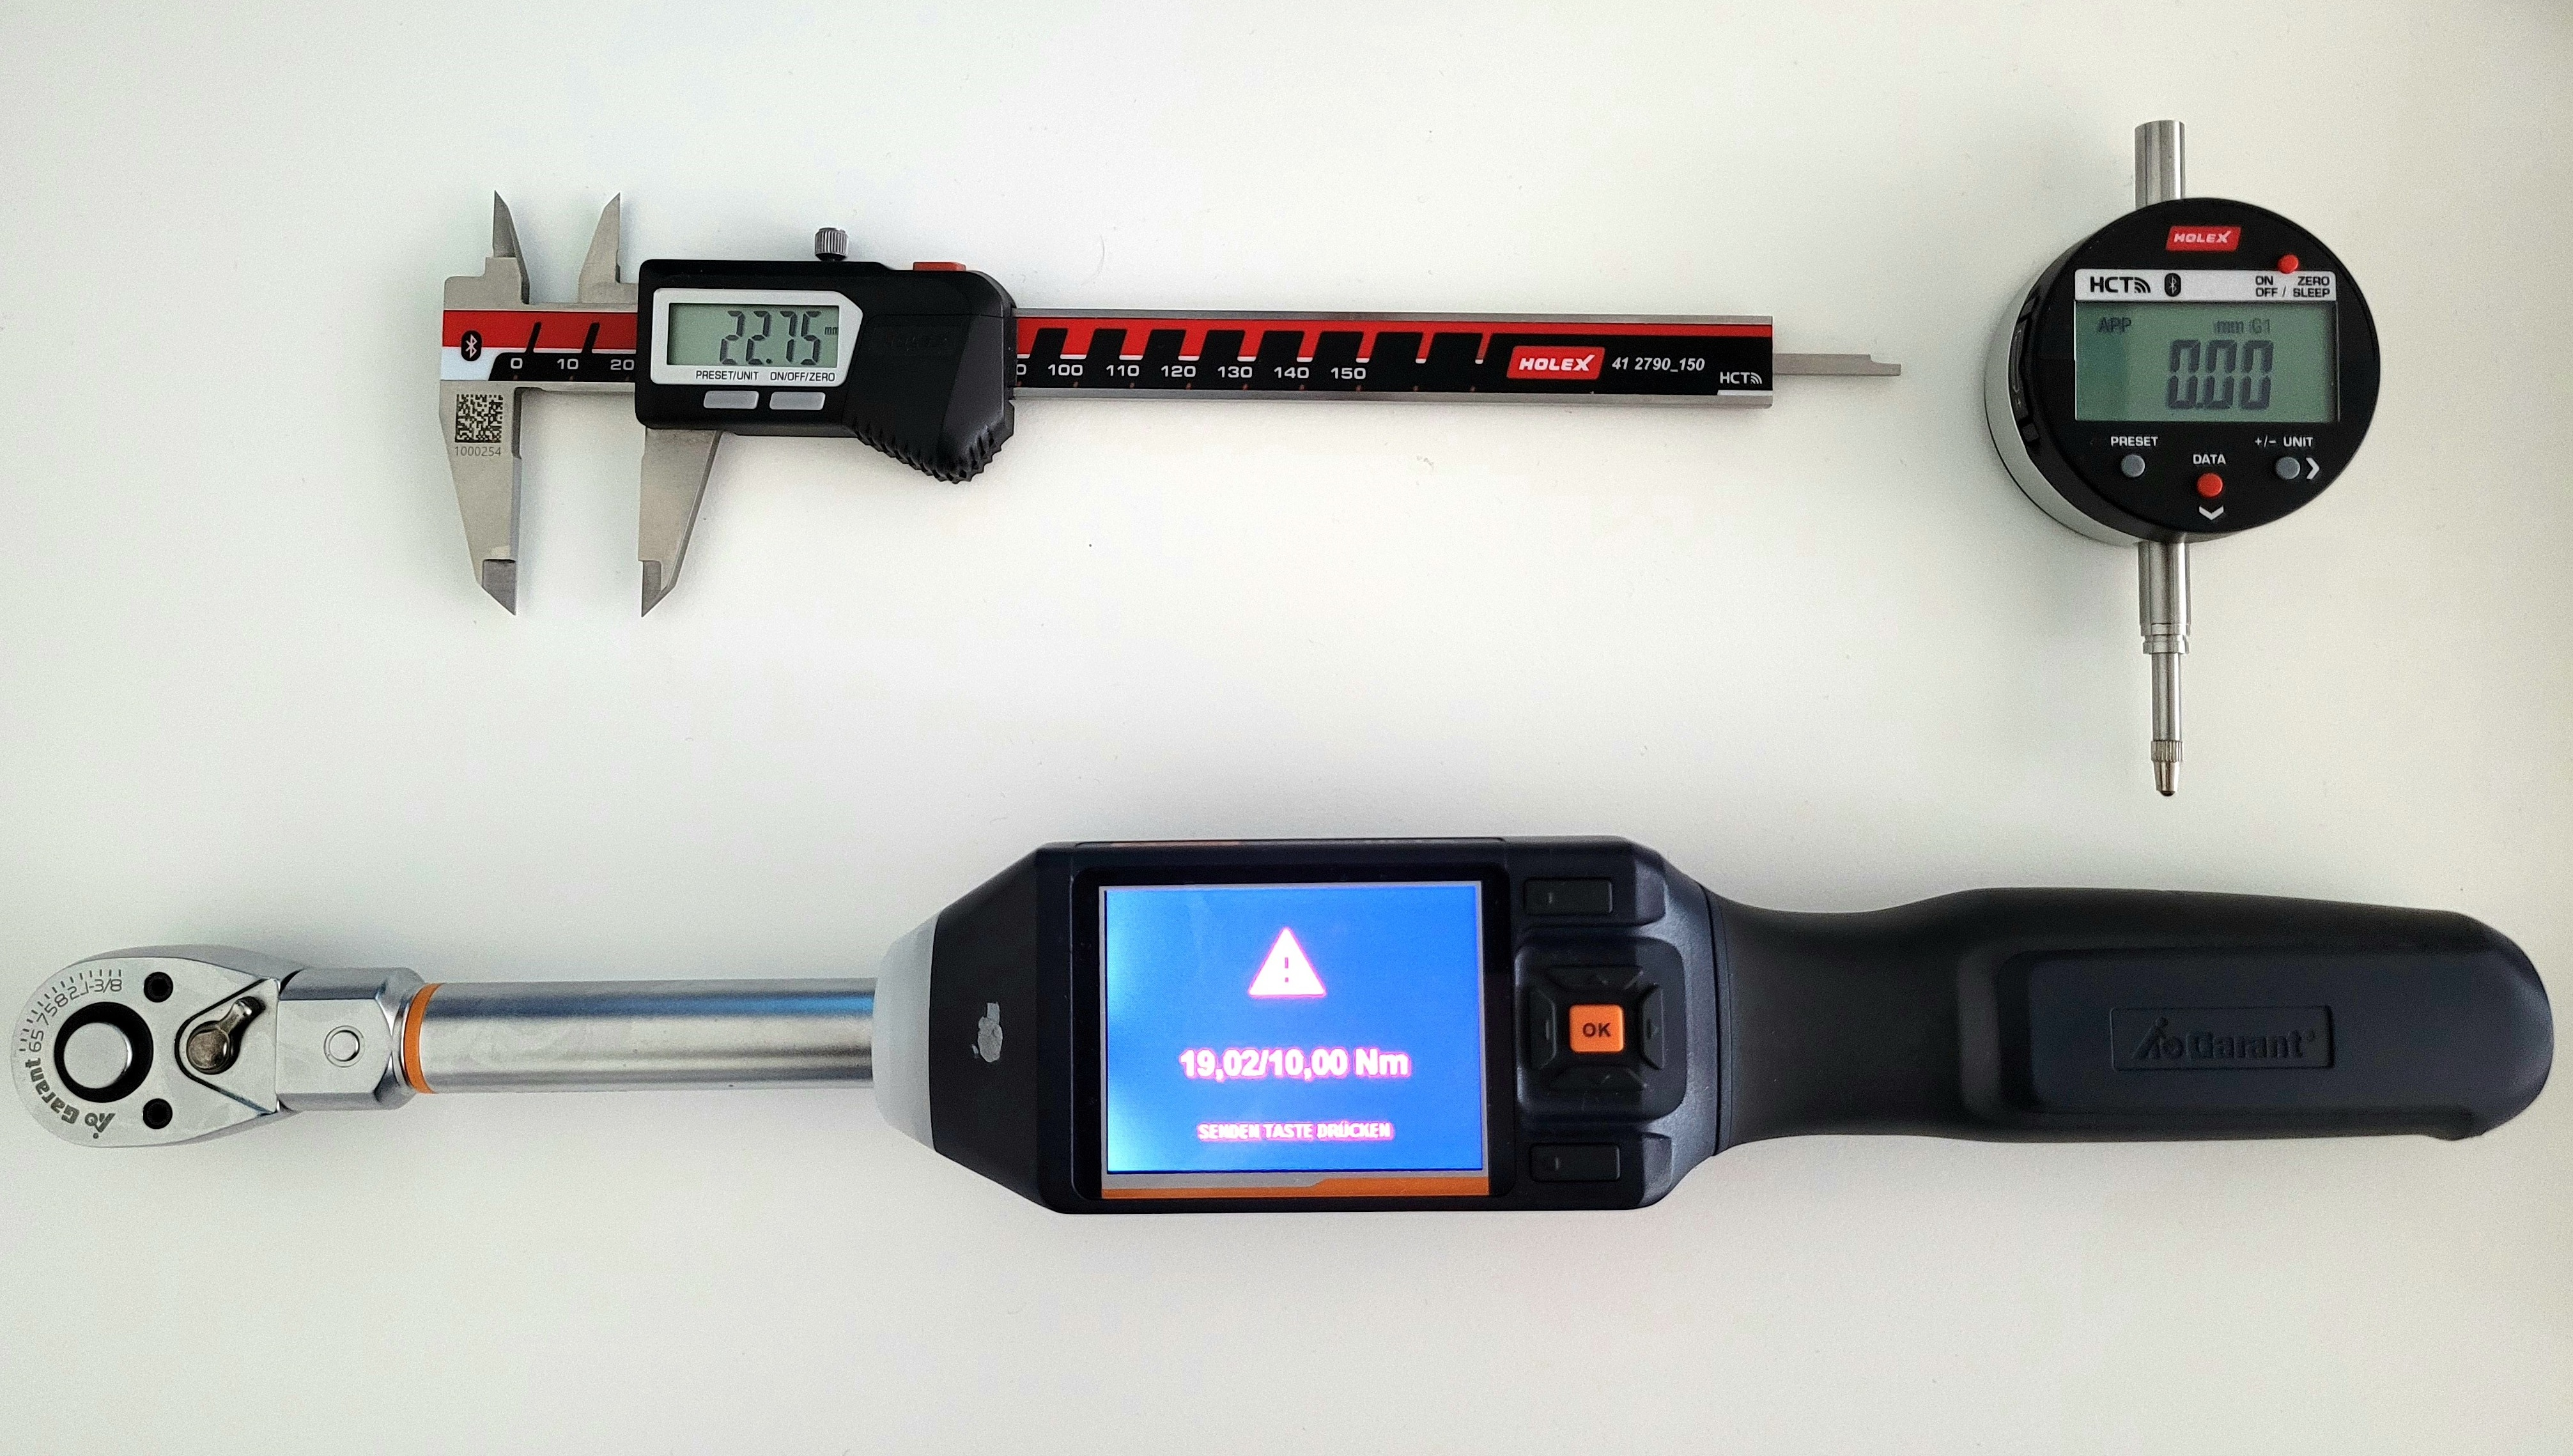
\includegraphics[width=\textwidth]{figures/Messmittel.jpg}
	\caption{Messmittel}
	\label{fig:Messmittel}
\end{figure}
Die Funktionalität des Fußtasters den Anwender zu befähigen ein Messergebnis zeitgenau und präzise auszulösen, hat bei der Art wie das Messergebnis bei Drehmomentschlüssel vorliegt, also keine besondere Bedeutung. Daher wurde die Entscheidung getroffen bei Betätigung des Fußtasters nicht das Messergebnis von Drehmomentschlüssel abzufragen, sondern die Funktionalität ganz auf Messuhren zuzuschneiden. Dabei ensteht das Problem, dass die ausgelösten Messergebnisse immer in der gleichen Reihenfolge ausgegeben werden müssen, um sie einer Messuhr zuordbar zu machen. Um dieses Problem zu lösen, wird eine spezielle Funktionalität entwickelt, die Gruppenfunktion. Die Mechanismen zur flexiblen Verarbeitung der Messdaten, sowie die Entwicklung der Gruppenfunktion werden in Kapitel \ref{EinbindungMessuhren} vorgestellt und anhand der Einbindung der Messuhren beziehungsweise Messschieber umgesetzt.

\subsection{Fußschalter Hardware}
Für den Fußschalter steht eine Reihe an Hardware Funktionen zur Verfügung. Deren Funktionalität muss evaluiert und eingebunden werden um die Funktionsweise der Anwendung sinnvoll zu ergänzen. Der Fußtaster stellt neben der Änderung der Konfigurationsdateien die einzige Möglichkeit für den Anwender dar, um mit dem Fußschalter zu interagieren, weshalb sein Funktionsumfang maximiert werden soll. Die Drei-Farben-LED soll den internen Zustand des Fußschalters anzeigen und Aufschluss über die Prozessvorgänge geben. In Abbildung \ref{fig:Fussschalter} ist der Fußschalter mit und ohne Abdeckung zu sehen. Der blaue, auf die Platine gelötete nRF-52840 Dongle ist zu sehen, ebenso wie der Akku und der Schalter für den Fußtaster.
\begin{figure}[H] 
	\centering
	\includegraphics[width=0.9\textwidth]{figures/Fußschalter.jpg}
	\caption{Der Fußschalter mit und ohne Abdeckung}
	\label{fig:Fussschalter}
\end{figure}
Wenn der Fußschalter nicht über \ac{USB} mit einer Stromquelle verbunden ist, bekommt er den benötigten Strom von der fest eingebauten Batterie. Um diese nicht unnötig zu belasten, muss ein Energiemanagement geschaffen werden, dass die bestehenden Ressourcen optimiert. Die Erhöhung der Effizienz der Batterienutzung kann dabei auf zwei Weisen erreicht werden. Einerseits kann bei Nutzung des Fußschalter die Energieeffizienz verbessert werden, was in Kapitel \ref{OptimierungAbfrage} mit einer Optimierung der Abfrage der Messeinheit umgesetzt wird. Andererseits kann bei Inaktivität des Fußschalters dessen Funktionalität abgeschaltet werden, um ebenfalls die Laufzeit der Batterie zu verlängern. Dazu muss festgelegt werden was Inaktivität bedeutet und nach welcher Zeit der Inaktivität drastische Stromsparmaßnahmen, wie das vollständige Ausschalten des Fußtasters, erfolgen.\\
Inaktivität als solche muss klar definiert werden, da sie einerseits programmatisch festgestellt werden soll und andererseits gewisse Aktivitäten, wie eine aktive Verbindung, nicht unbedingt darauf hindeuten, dass der Fußschalter tatsächlich in Gebrauch ist. Anstatt alle Tätigkeiten des Fußschalters zu kategorisieren, wird stattdessen festgelegt welche Ereignisse ein Herunterfahren des Geräts verhindern sollen. Diese sind zum Ende der Arbeit einerseits das Erhalten eines Messergebnisses und andererseits der angestoßene Verbindungsaufbau zu einem Werkzeug.\\
Für die Dauer der Inaktivität, nach der der Fußschalter heruntergefahren werden soll, kann keine allgemeingültige Aussage getroffen werden. Da eine angemessene Zeitdauer von persönlichen Präferenzen und dem Anwendungsfall abhängt. Daher wird sich an dieser Stelle entschieden, die Zeitdauer durch den Anwender konfigurierbar zu machen. Dazu wurde in der Konfigurationsdatei config.ini ein Attribut angelegt, durch das der Anwender die Zeit, nach der das Gerät heruntergefahren wird, in Sekunden angeben kann.